\documentclass[aps,prd,onecolumn,nofootinbib,superscriptaddress]{revtex4-2}

% ----------------------------------------
% Packages
% ----------------------------------------
\usepackage[utf8]{inputenc}
\usepackage[T1]{fontenc}
\usepackage{lmodern}
\usepackage{amsmath,amssymb,amsfonts,bm}
\usepackage{graphicx}
\usepackage{xcolor}
\usepackage{hyperref}
\usepackage{siunitx}
\usepackage{enumitem}

\hypersetup{
  colorlinks=true,
  linkcolor=blue,
  citecolor=blue,
  urlcolor=blue
}

% ----------------------------------------
% Shortcuts
% ----------------------------------------
\newcommand{\Mpl}{M_{\rm Pl}}
\newcommand{\Meff}{M_{\rm eff}}
\newcommand{\Om}{\Omega}
\newcommand{\dd}{\mathrm{d}}
\newcommand{\trm}{\mathrm}
\newcommand{\etal}{\textit{et al.}}

\begin{document}

\title{TCV-$\phi$ II: cohesive bounce, geometric reheating,\
and baseline baryogenesis/ULDM pipelines}

\author{Cyrille LECROQ}
\affiliation{Independent Researcher}

\date{2025}

\begin{abstract}
This second paper develops the next conservative step of the TCV-$\phi$ programme, using the same two-scalar EFT defined in Paper~I and keeping all Paper~I conventions and benchmark scales fixed unless explicitly stated.
Our scope is to build and document the working numerical pipelines for (i) an illustrative cohesive-bounce background, (ii) a geometric-reheating mapping, (iii) a baseline spontaneous-baryogenesis estimator sourced by $\dot\Phi_1$, and (iv) a refined homogeneous ULDM treatment for $\Phi_2$.
At this stage, the bounce profile and reheating/baryogenesis mappings are treated as controlled phenomenological ans\"atze compatible with the EFT, not as unique derivations from first principles.
On the Boltzmann side, we provide a clean interface layer that supports both standard power-law primordial inputs and an external tabulated primordial spectrum, with explicit diagnostics for CLASS calls.
A full likelihood-level confrontation to CMB/LSS data and a full perturbative derivation of the ULDM and primordial sectors are deferred to the subsequent dedicated paper.
\end{abstract}

\maketitle

% ----------------------------------------
\section{Introduction}
% ----------------------------------------

Paper~I established the minimal TCV-$\phi$ effective field theory (EFT): gravity plus two real scalar fields, a heavy structural mode $\Phi_1$, a light coherent mode $\Phi_2$, and a mildly non-minimal Planck mass $\Meff^2(\Phi_1)$ that is effectively constant for late-time cosmology.
In that first step, the focus was intentionally limited to a $\Lambda$CDM-like homogeneous background and an illustrative ULDM-like suppression template for the matter power spectrum.

The objective of the present paper is different: we organize, stabilize, and benchmark the computational pipeline needed for the next physics layers of the programme, while keeping the same conservative writing standard and the same EFT conventions.
The aim is not to claim a revolutionary phenomenology at this stage, but to build a technically clean and testable path from the canonical Paper~I EFT toward a broader cohesive-cosmology interpretation.
In particular, this paper establishes the \emph{Paper~II computational backbone}:
\begin{enumerate}[label=(\roman*),leftmargin=1.5em]
  \item an explicit cohesive-bounce background module;
  \item a geometric-reheating mapping that outputs post-bounce initial conditions;
  \item a baseline spontaneous-baryogenesis module based on a derivative coupling to $\Phi_1$;
  \item a refined homogeneous ULDM treatment for $\Phi_2$ plus a cleaner Boltzmann interface for future data-driven analyses.
\end{enumerate}

It is important to state clearly what is and is not claimed here.
We do \emph{not} claim a full microphysical derivation of the bounce profile, nor a precision baryogenesis fit, nor a final perturbative ULDM implementation in Einstein--Boltzmann solvers.
Instead, we provide reproducible modules, diagnostics, and benchmark outputs that are consistent with the EFT and directly reusable in the next PRD-stage paper.

Throughout this paper we use natural units $c=\hbar=1$ and the reduced Planck mass $\Mpl\simeq 2.435\times10^{18}\,\trm{GeV}$.

% ----------------------------------------
\section{EFT baseline and benchmark conventions}
\label{sec:eft-baseline}
% ----------------------------------------

We keep exactly the same baseline EFT structure as in Paper~I,
\begin{align}
S &= \int \dd^4x\,\sqrt{-g}
\left[
\frac{1}{2}\Meff^2(\Phi_1)R
-\frac12(\nabla\Phi_1)^2
-\frac12(\nabla\Phi_2)^2
-V(\Phi_1,\Phi_2)
\right]
+S_{\rm SM},
\end{align}
with
\begin{align}
\Meff^2(\Phi_1)&=\Mpl^2\left(1+\xi_0\frac{\Phi_1^2}{\Mpl^2}\right),
\\
V(\Phi_1,\Phi_2)&=V_1(\Phi_1)+V_2(\Phi_2)+\rho_{\rm vac},
\end{align}
and the Paper~I benchmark scale hierarchy $m_1\gg m_2$.

In this paper we add only \emph{operational} parameters required by the new modules (e.g. bounce time scale, reheating efficiency, baryogenesis scale $\Lambda_B$), and we explicitly keep them in the phenomenological layer.
No redefinition of the Paper~I microscopic parameter set is introduced.

% ----------------------------------------
\section{Cohesive bounce and geometric reheating module}
\label{sec:bounce}
% ----------------------------------------

\subsection{Background ansatz and structural-field evolution}

The current bounce module uses the standard symmetric template
\begin{equation}
a(\eta)=a_b\sqrt{1+\left(\frac{\eta}{\eta_0}\right)^2},
\label{eq:bounce-ansatz}
\end{equation}
with conformal time $\eta$.
Given this background, the homogeneous structural field is evolved with
\begin{equation}
\Phi_1''+2\frac{a'}{a}\Phi_1'+a^2\,\partial_{\Phi_1}V_1=0,
\end{equation}
using the benchmark potential inherited from Paper~I.
For the benchmark run shown below, the initial conditions used in the code are
\begin{equation}
\Phi_1(\eta_{\rm min})=\Phi_0(1+10^{-3}),
\qquad
\Phi_1'(\eta_{\rm min})=0,
\end{equation}
with $(\eta_{\rm min},\eta_{\rm max})=(-50,50)$, matching the benchmark script configuration.

At this stage Eq.~\eqref{eq:bounce-ansatz} is an explicit phenomenological ansatz used to generate a controlled numerical history.
It is suitable for pipeline validation, but it is not presented as a unique EFT prediction.

\begin{figure}[t]
  \centering
  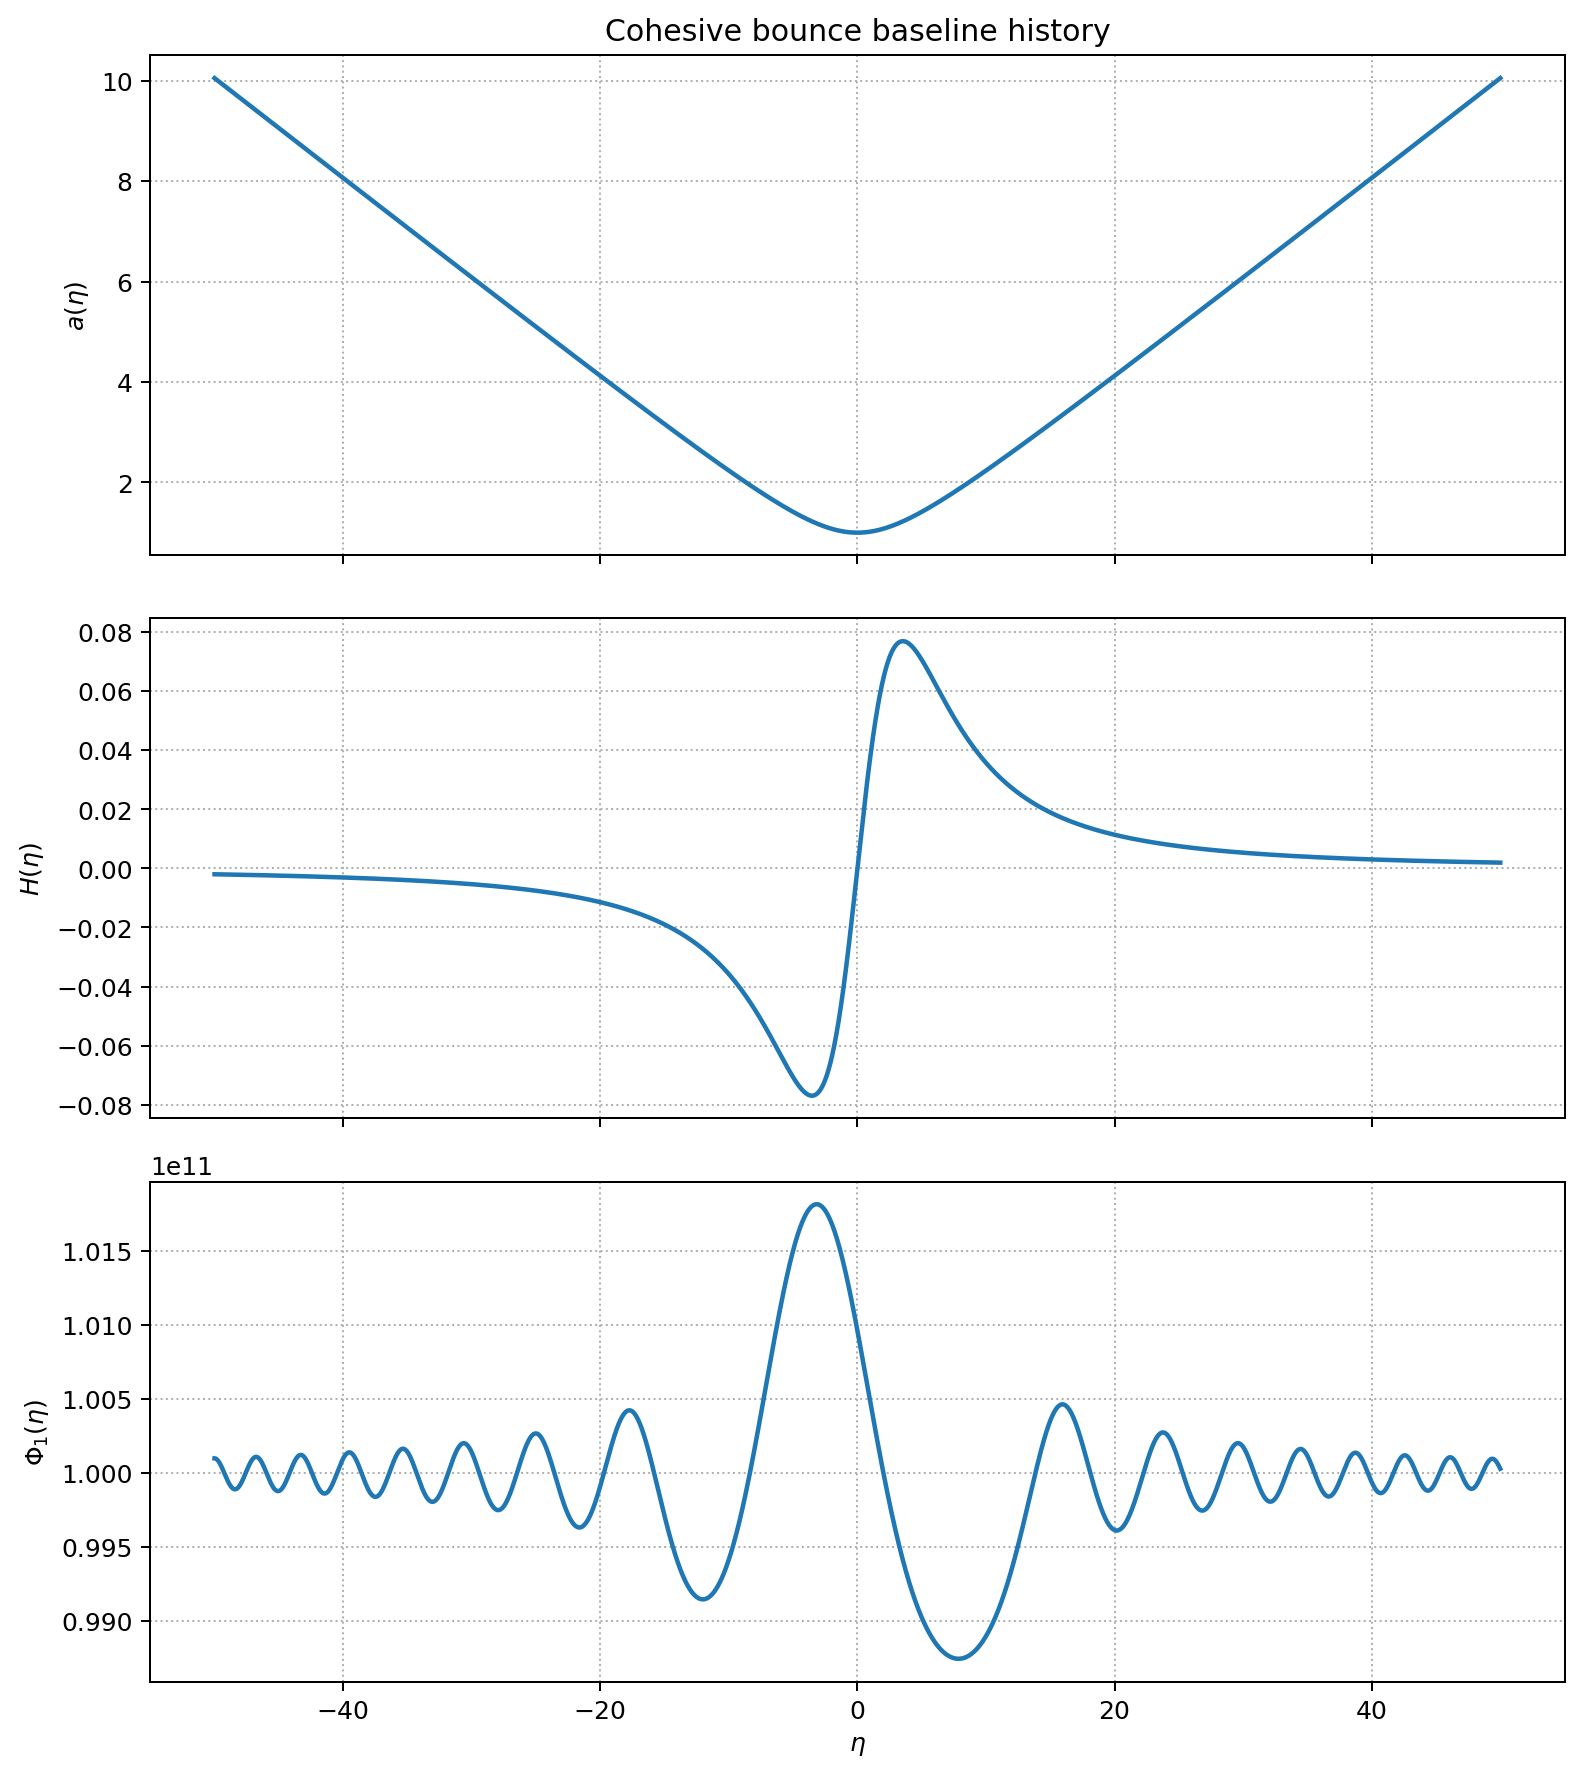
\includegraphics[width=0.82\textwidth]{../figs/bounce_history_background.png}
  \caption{Illustrative cohesive-bounce benchmark history generated by \texttt{compute\_bounce\_history.py}: scale factor $a(\eta)$, Hubble history, and structural field evolution.}
  \label{fig:bounce-background}
\end{figure}

\subsection{Geometric reheating map}

The numerical module then maps a fraction of the structural-sector energy into an effective radiation component and defines a reheating scale from
\begin{equation}
\rho_r=\frac{\pi^2}{30}g_*T^4.
\end{equation}
In the benchmark implementation, we use $g_*=106.75$, a reheating-efficiency parameter
$\epsilon_{\rm reh}=0.8$, and the reference reheating time $\eta_{\rm reh}=2\,\eta_0$.
For the current benchmark run, this gives
\begin{equation}
T_{\rm reh}\simeq 3.1\times10^9\,\trm{GeV},
\end{equation}
with explicit energy-ratio diagnostics exported in
\texttt{papers/paper-02/data/bounce\_summary.json}.

\begin{figure}[t]
  \centering
  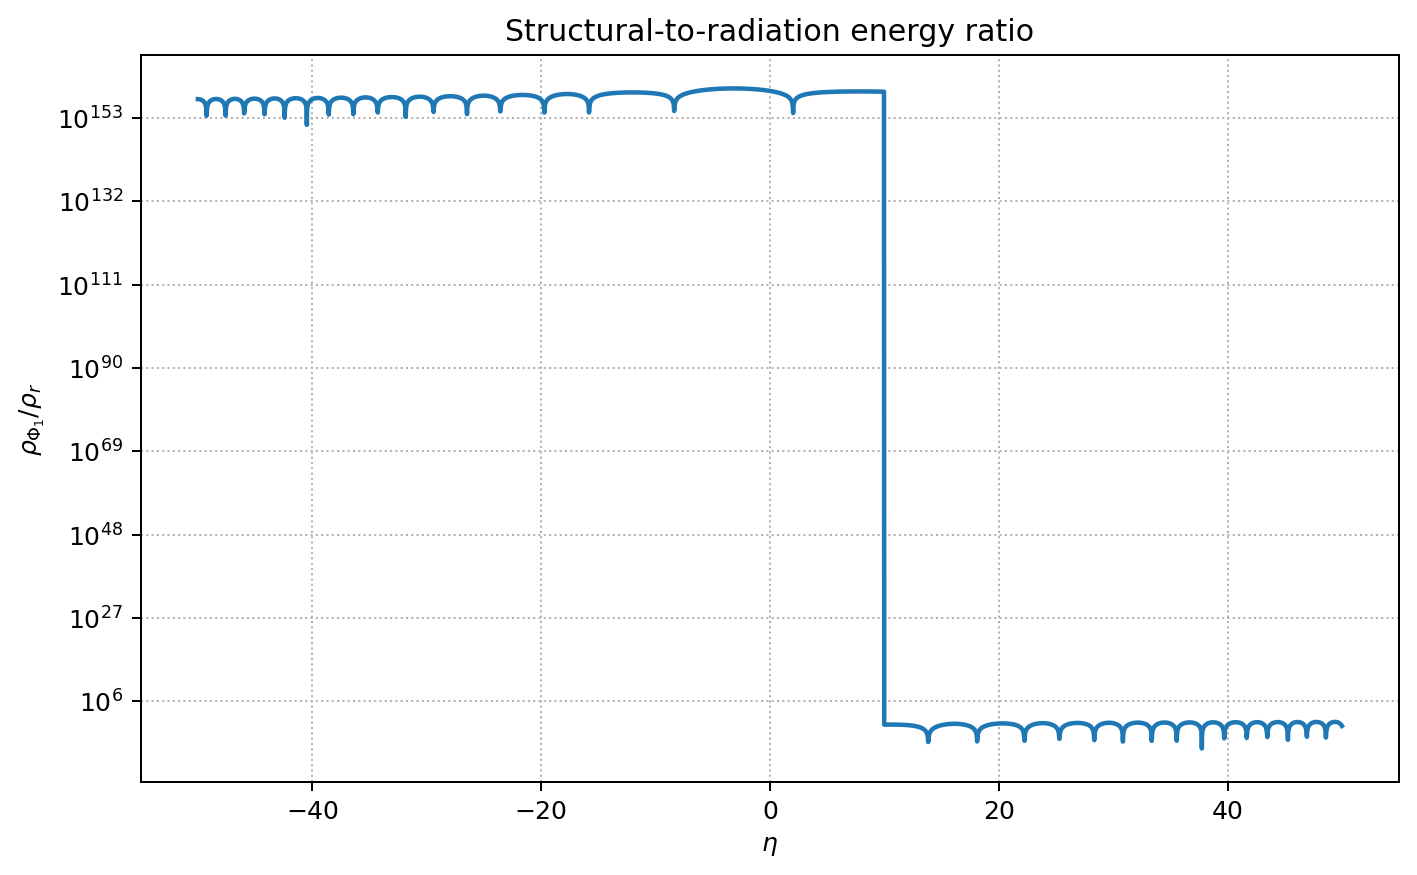
\includegraphics[width=0.72\textwidth]{../figs/bounce_history_energy_ratio.png}
  \caption{Benchmark energy-ratio diagnostics from the bounce/reheating run. This figure is used as a numerical consistency check of the pipeline rather than as a precision observable.}
  \label{fig:bounce-energy}
\end{figure}

% ----------------------------------------
\section{Baseline spontaneous baryogenesis module}
\label{sec:baryo}
% ----------------------------------------

The current baryogenesis layer implements a derivative interaction of the form
\begin{equation}
\frac{\partial_\mu\Phi_1}{\Lambda_B^2}J_B^\mu,
\end{equation}
which induces an effective chemical potential
\begin{equation}
\mu_B\sim\frac{\dot\Phi_1}{\Lambda_B^2}.
\end{equation}
A freeze-out temperature is estimated from $\Gamma_B(T_B)\sim H(T_B)$ with the explicit rate model
\begin{equation}
\Gamma_B(T)=\alpha_B\,\frac{T^{p}}{\Lambda_B^{q}},
\qquad
(\alpha_B,p,q)=(0.1,5,4)
\end{equation}
used in the benchmark code.

This module is currently a baseline estimator: it provides a clean mapping from bounce histories to $(T_B,\eta_B)$ diagnostics and exposes which assumptions control the output.
The resulting benchmark values are saved in
\texttt{papers/paper-02/data/baryogenesis\_summary.json}.

\begin{figure}[t]
  \centering
  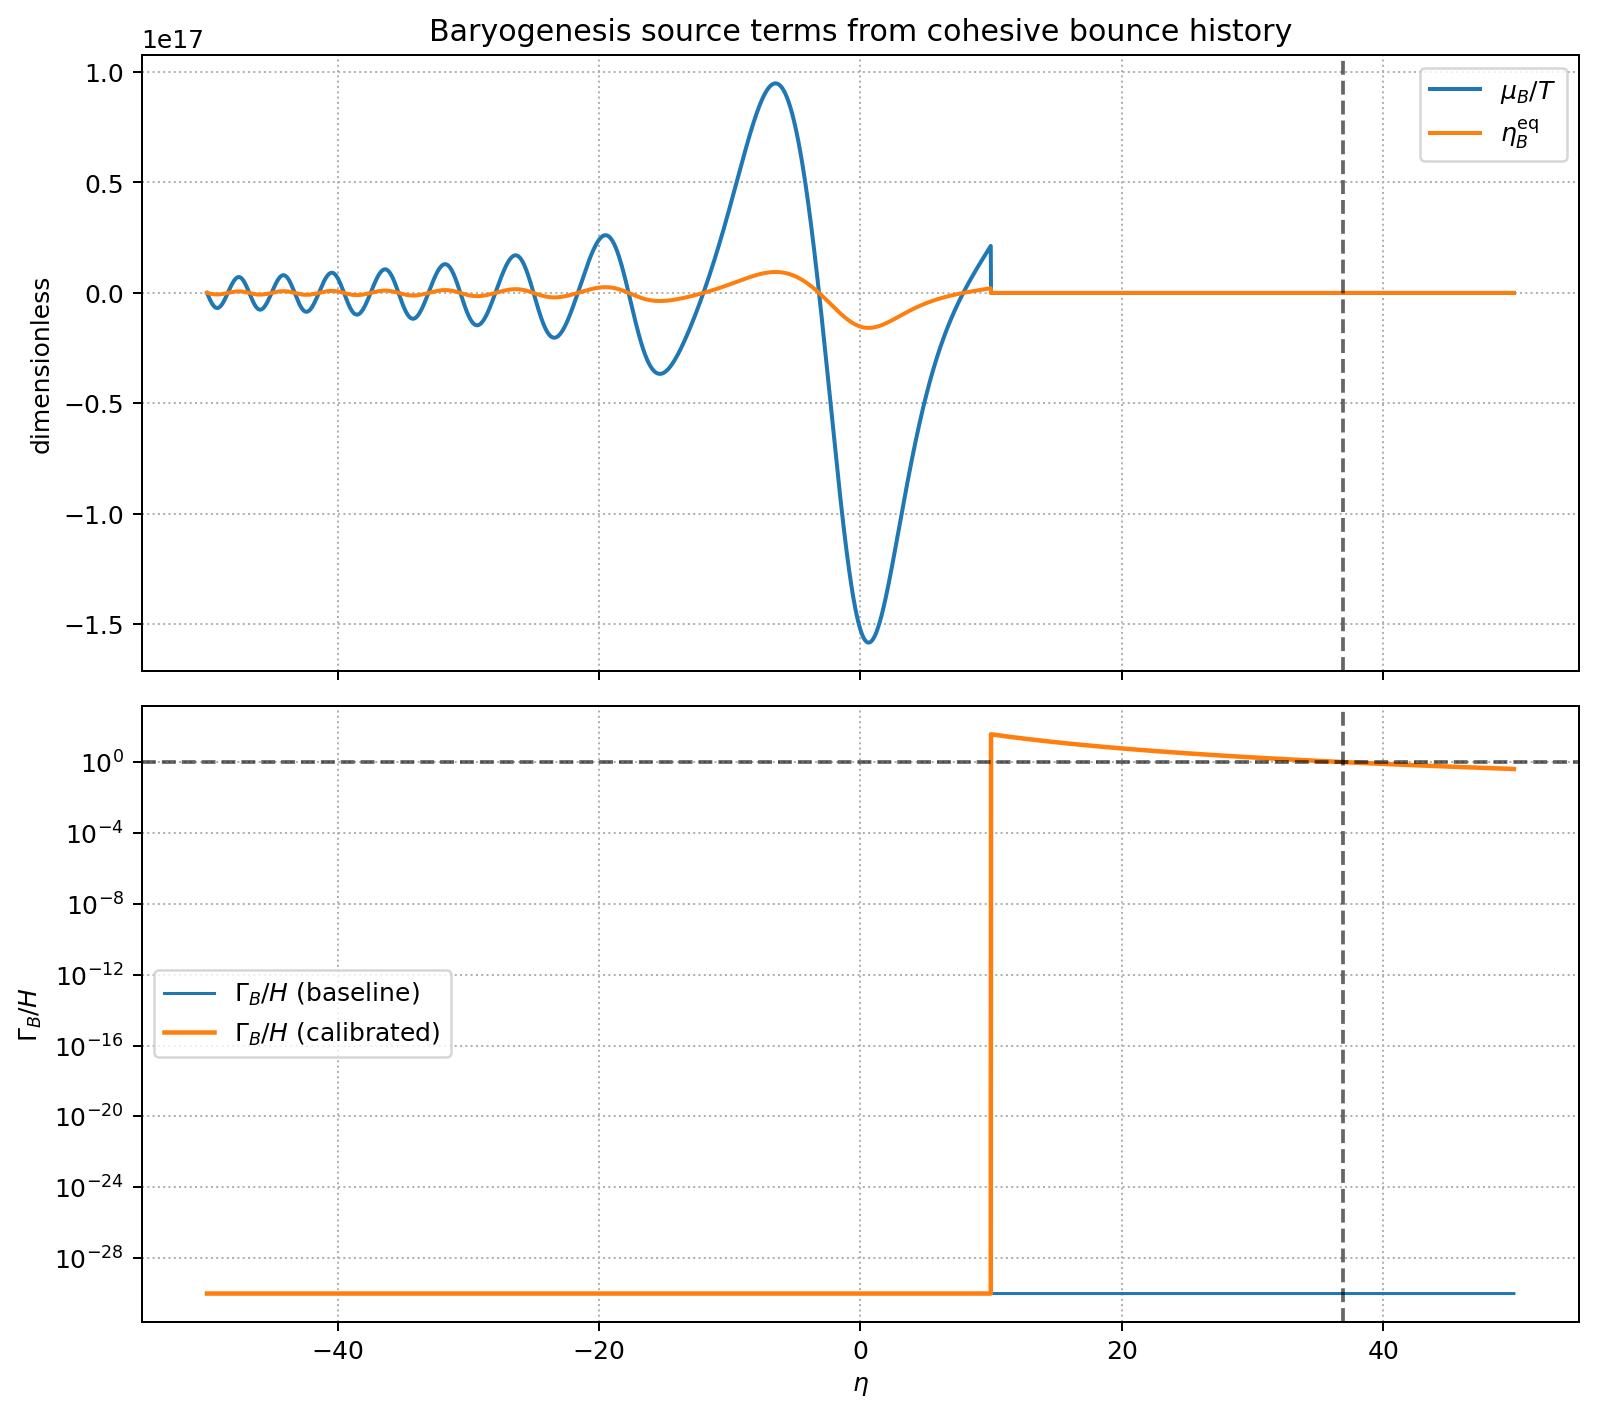
\includegraphics[width=0.72\textwidth]{../figs/baryogenesis_history.png}
  \caption{Example output of \texttt{compute\_baryogenesis.py}: thermal and rate diagnostics across the post-bounce history.}
  \label{fig:baryogenesis}
\end{figure}

% ----------------------------------------
\section{ULDM $\Phi_2$ background and effective perturbative bridge}
\label{sec:uldm}
% ----------------------------------------

\subsection{Homogeneous dynamics and scaling check}

For the coherent field $\Phi_2$ we solve
\begin{equation}
\ddot\Phi_2+3H\dot\Phi_2+m_2^2\Phi_2=0,
\label{eq:phi2-kg}
\end{equation}
with misalignment-type initial conditions.
The benchmark diagnostic confirms the expected late-time matter-like scaling,
\begin{equation}
\rho_{\Phi_2}\propto a^{-3},
\end{equation}
with fitted slope close to $-3$ in
\texttt{papers/paper-02/data/uldm\_summary.json}.

\begin{figure}[t]
  \centering
  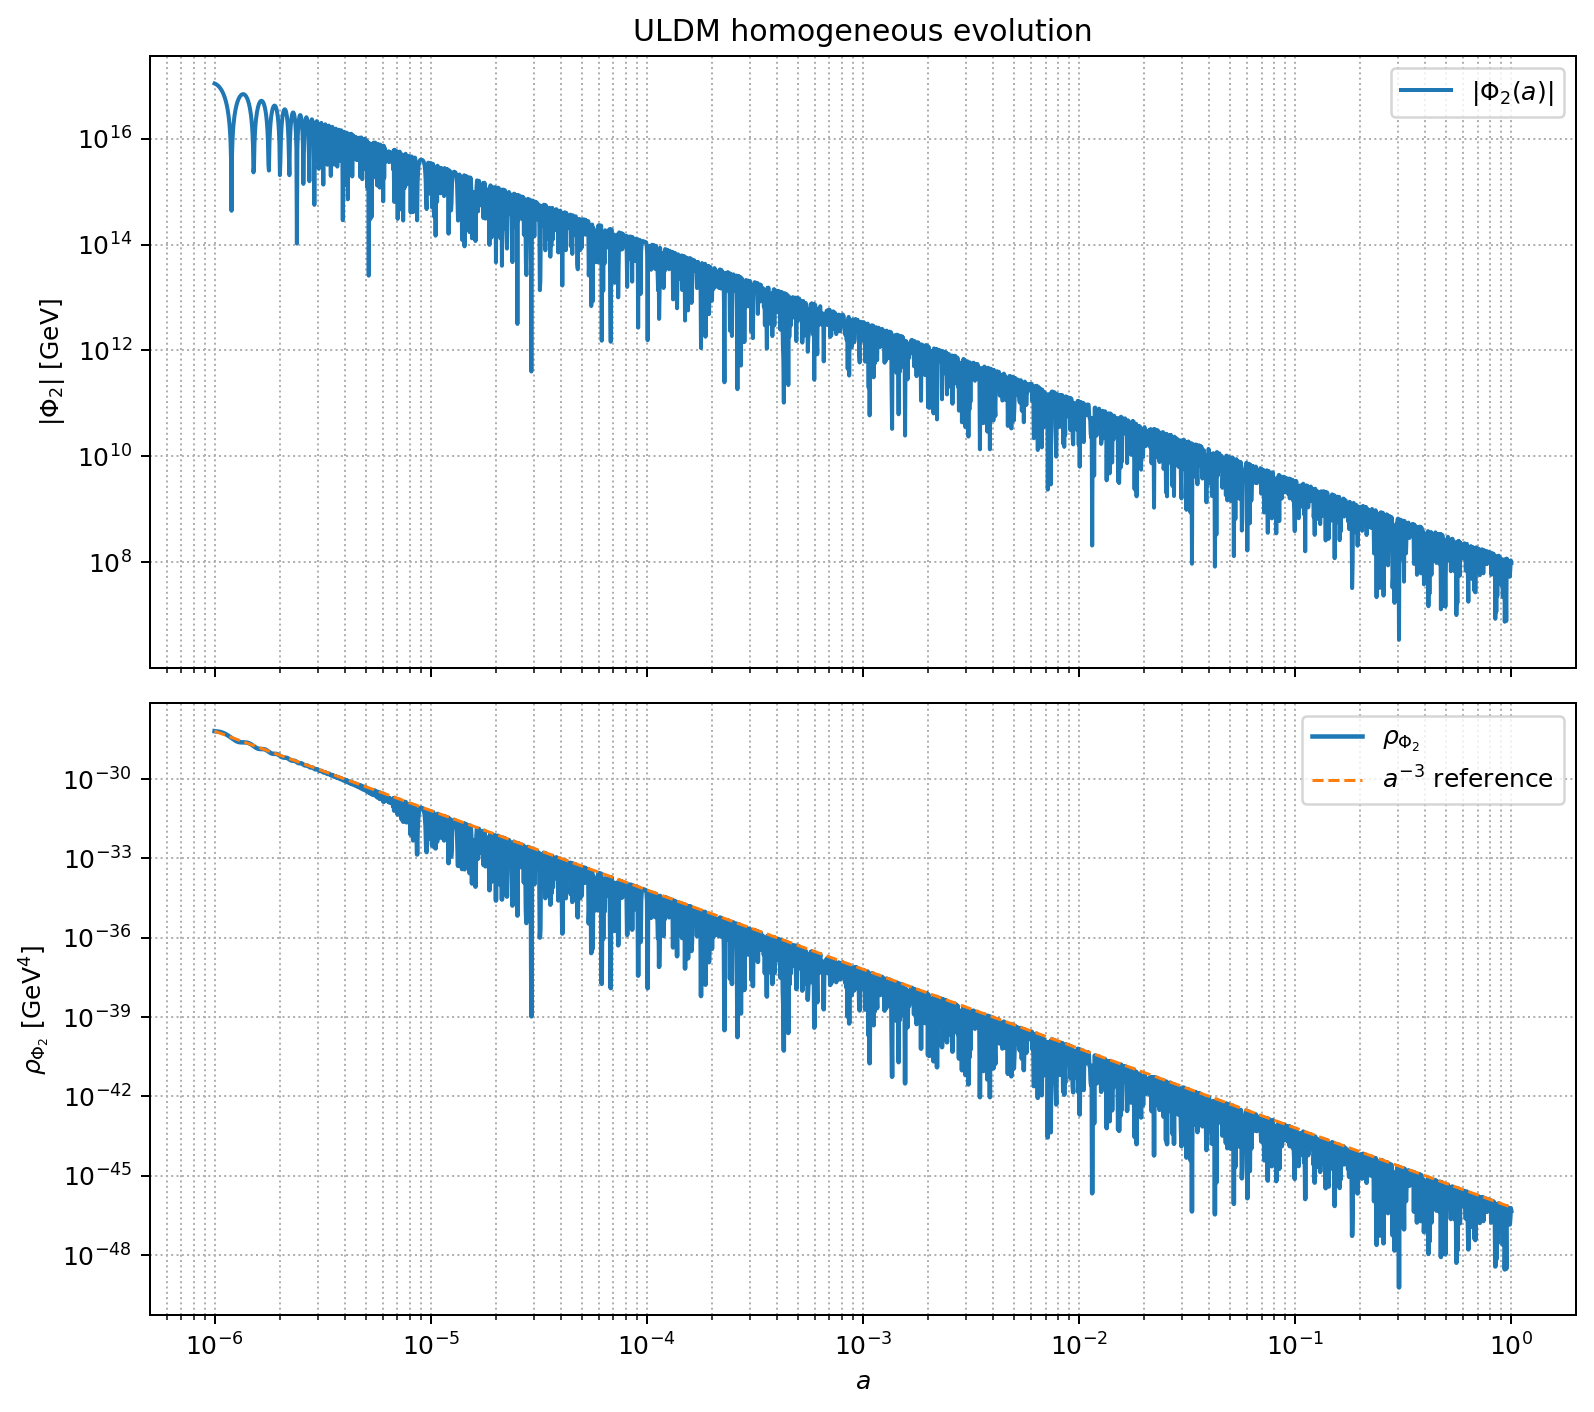
\includegraphics[width=0.72\textwidth]{../figs/uldm_background_scaling.png}
  \caption{Homogeneous ULDM benchmark diagnostic for $\Phi_2$. The late-time scaling approaches the expected matter-like behaviour.}
  \label{fig:uldm-background}
\end{figure}

\subsection{Current status of perturbations and Boltzmann coupling}

At this paper stage, the ULDM perturbation layer is still represented by an effective bridge to the existing CLASS workflow.
This is intentional: it preserves backward compatibility with Paper~I while preparing the transition to a full perturbative ULDM treatment.
Hence, the current $P(k)$ comparisons are interpreted as integration checks, not as final ULDM constraints.

\begin{figure}[t]
  \centering
  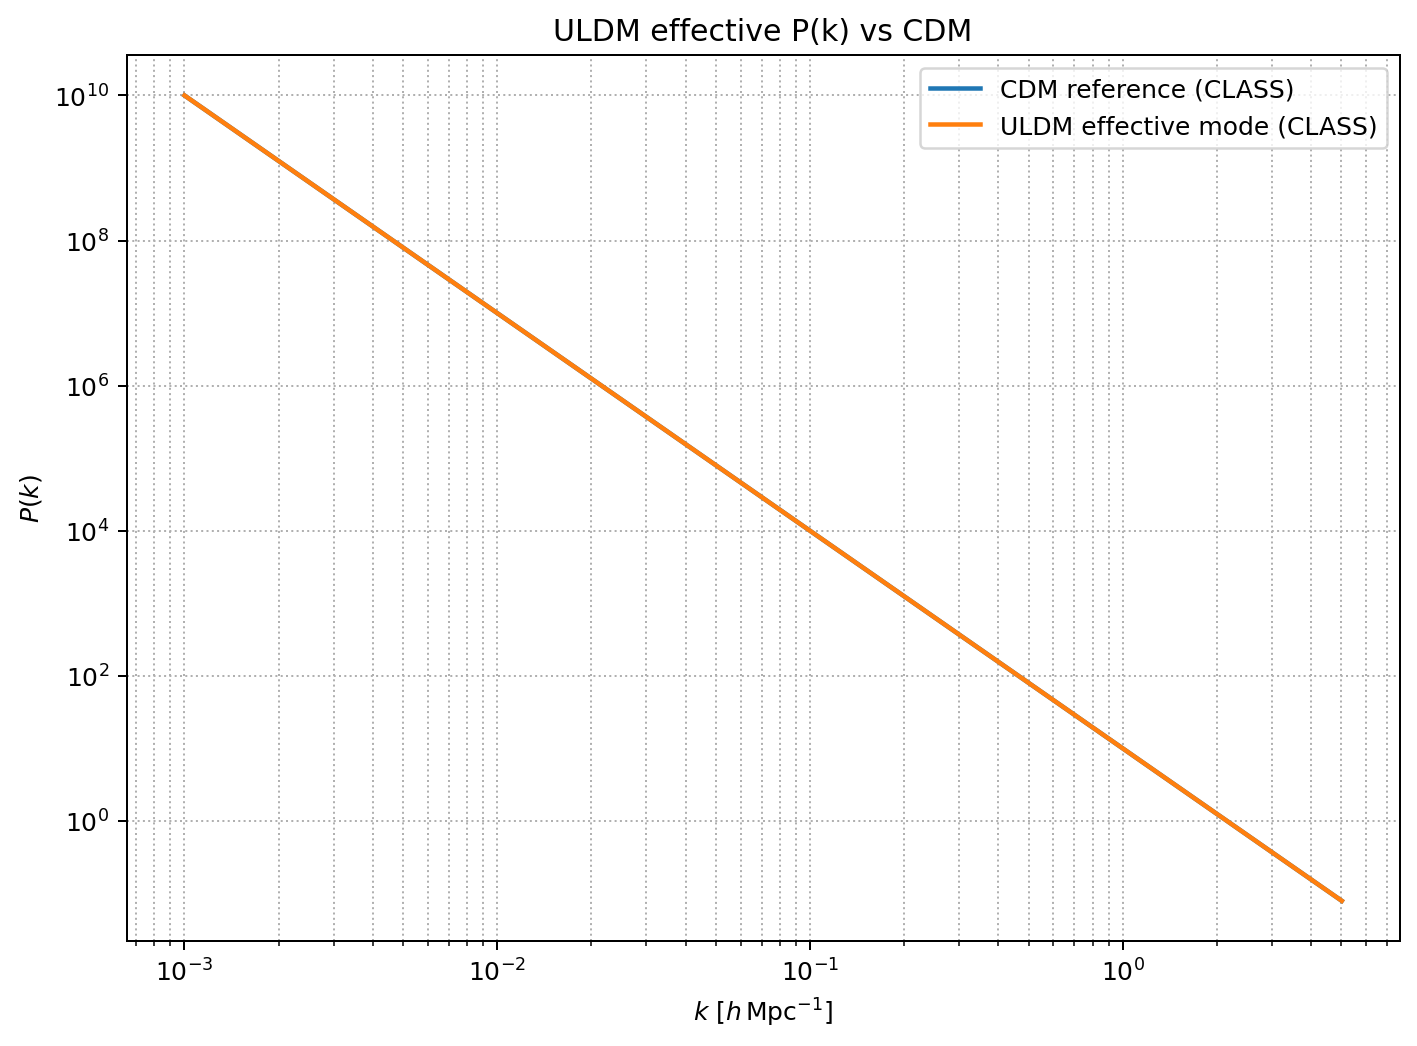
\includegraphics[width=0.72\textwidth]{../figs/uldm_pk_comparison.png}
  \caption{Current ULDM-vs-CDM comparison output from \texttt{compute\_uldm\_spectrum.py}. In the present implementation this figure is used only to validate the interface path, not to claim new data-level bounds: in this placeholder mode the ULDM branch is represented as effective CDM with the same benchmark density, so the ratio is expected to stay close to unity by construction.}
  \label{fig:uldm-pk}
\end{figure}

% ----------------------------------------
\section{Primordial spectrum pipeline and CLASS/CAMB interface status}
\label{sec:primordial}
% ----------------------------------------

The primordial module currently generates a tabulated spectrum $\mathcal{P}_\mathcal{R}(k)$ from a bounce-based pipeline and writes it to
\texttt{papers/paper-02/code/data/PR\_tcvphi.dat} (mirrored under \texttt{papers/paper-02/data/}).
The Boltzmann interface then supports two modes:
\begin{enumerate}[label=(\alph*),leftmargin=1.5em]
  \item standard power-law primordial input $(A_s,n_s)$;
  \item external primordial table mode.
\end{enumerate}
For the benchmark run we solve the Mukhanov--Sasaki equation
\begin{equation}
v_k''+\left(k^2-\frac{z''}{z}\right)v_k=0,
\end{equation}
in an effective cohesive-mixture model where
\begin{equation}
a(\eta)\propto |\eta|^{p},\qquad
p=\frac{2}{1+3w_{\rm eff}},\qquad
z(\eta)=a(\eta)\,C(\eta),
\end{equation}
with a Lorentzian cohesive factor
\begin{equation}
C(\eta)=1+\frac{C_0}{1+(\eta/\eta_c)^2}.
\end{equation}
The corresponding benchmark parameters are
\begin{equation}
w_{\rm eff}=-0.003,\qquad C_0=-0.0038,\qquad \eta_c=50,\qquad \texttt{mode}=\texttt{lorentzian}.
\end{equation}
In the current benchmark pipeline, the tabulated spectrum is then rescaled so that its amplitude matches the target $A_s=2.1\times10^{-9}$ at the pivot scale.
This primordial sector is therefore an explicit phenomenological ansatz used for pipeline validation, not yet a unique microphysical prediction of the EFT.

For the current benchmark run, the diagnostic summary indicates stable CLASS calls (no fallback) in both modes and a near-unity $P(k)$ ratio between the two interface routes over the tested range.
These are software-validation statements; the full perturbative and likelihood-level interpretation is postponed to the dedicated primordial paper.

\begin{figure}[t]
  \centering
  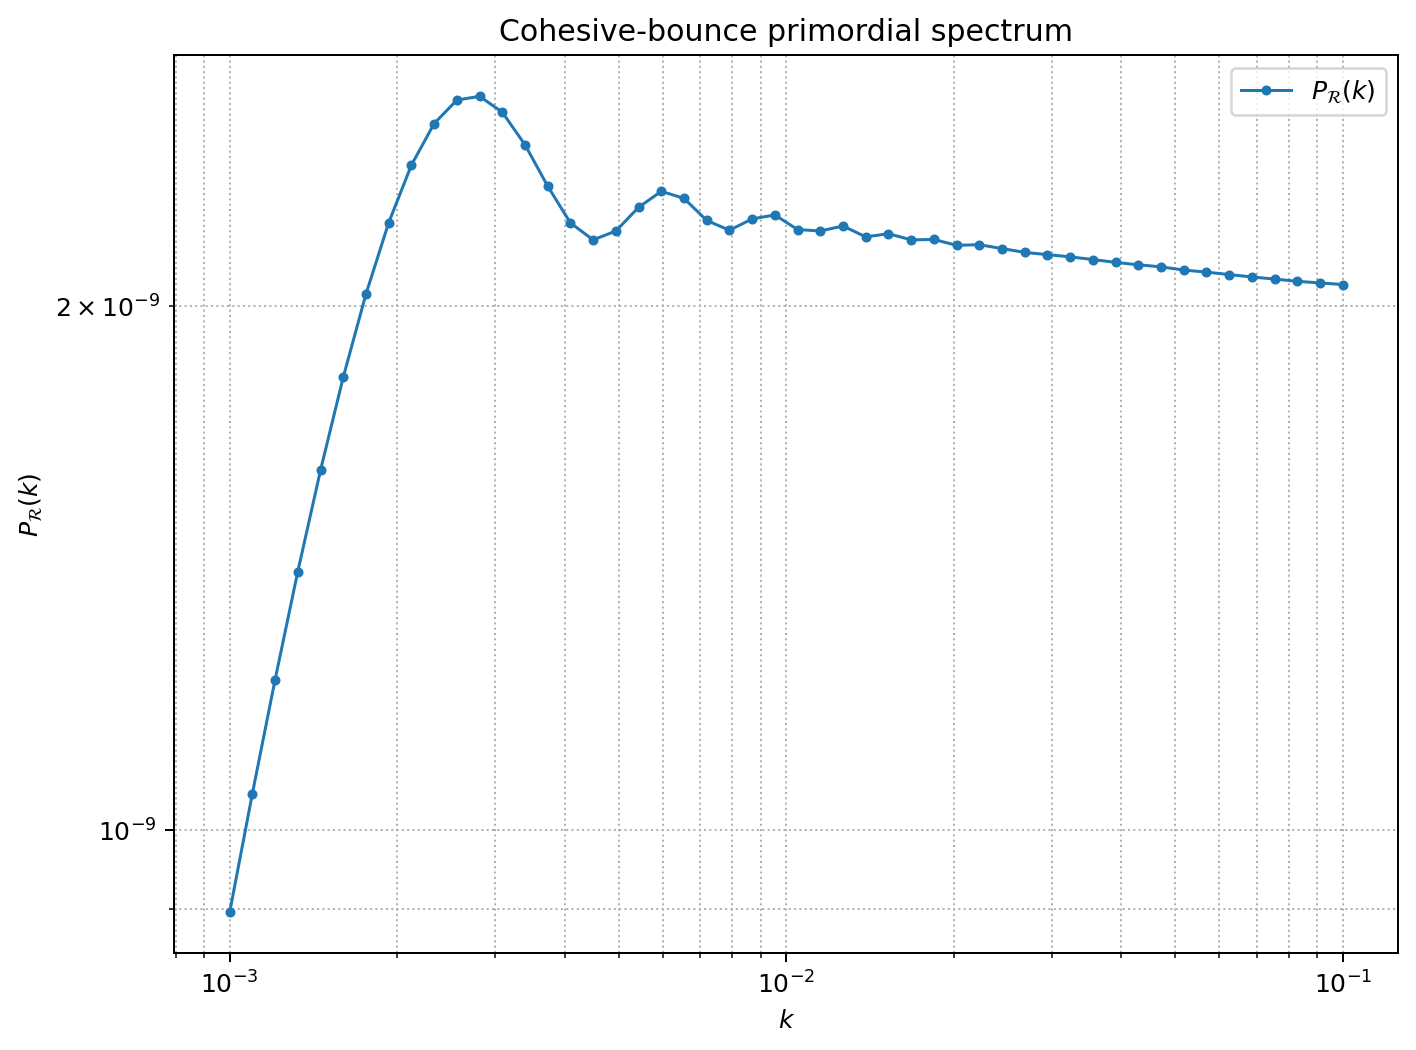
\includegraphics[width=0.72\textwidth]{../figs/primordial_spectrum.png}
  \caption{Illustrative primordial spectrum table generated by \texttt{compute\_primordial\_spectrum.py}.}
  \label{fig:primordial-spectrum}
\end{figure}

\begin{figure}[t]
  \centering
  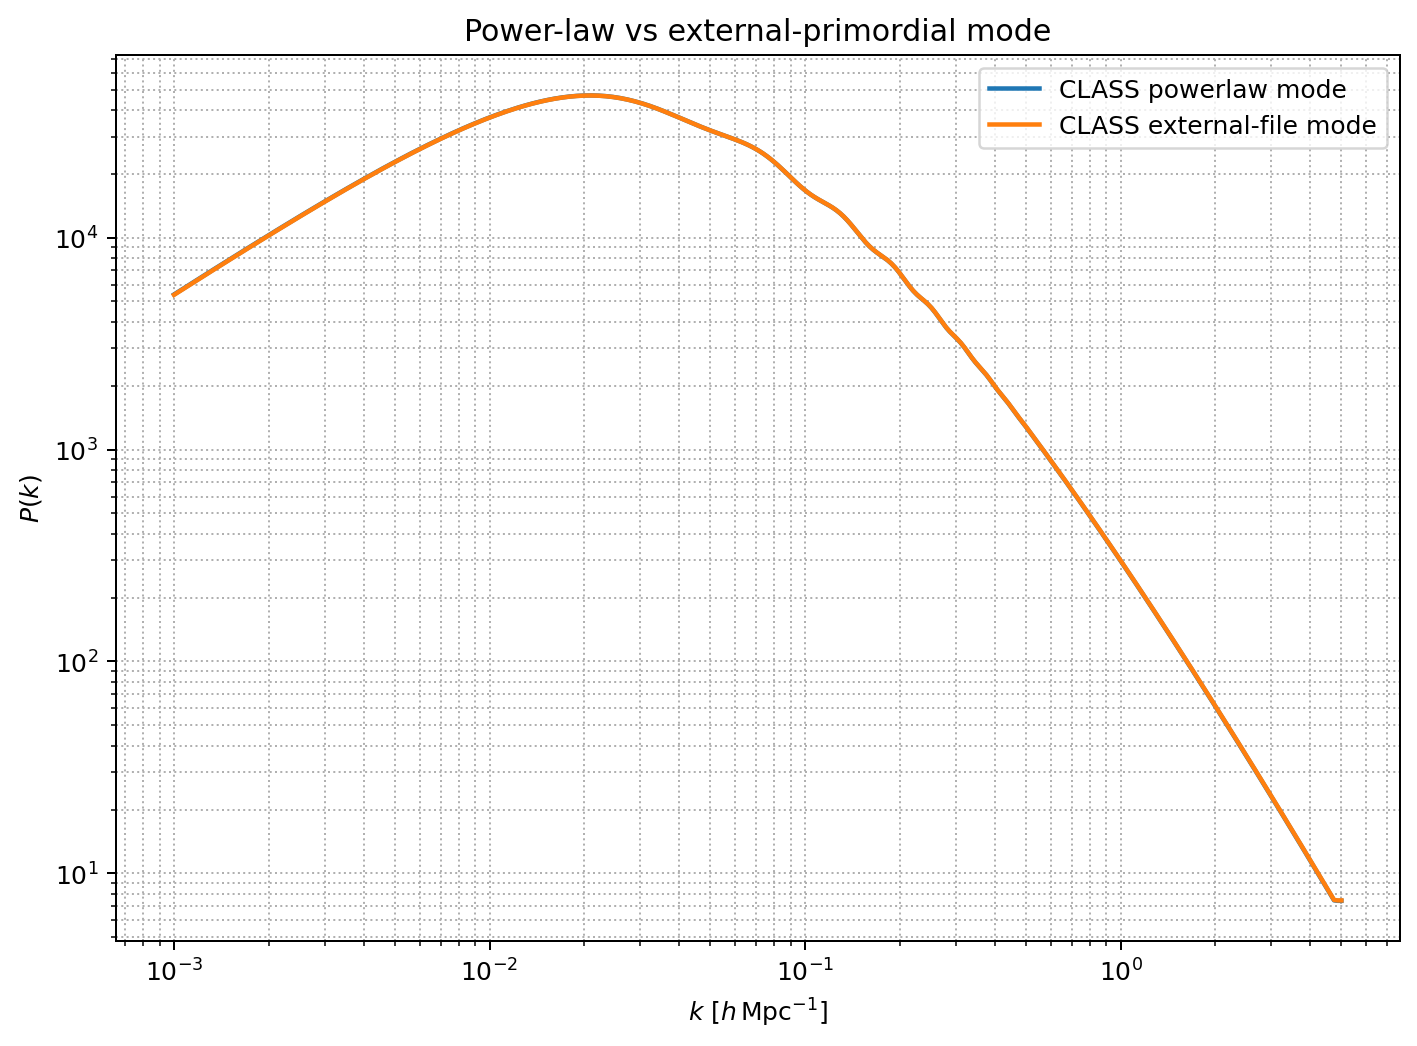
\includegraphics[width=0.72\textwidth]{../figs/primordial_pk_comparison.png}
  \caption{CLASS interface cross-check: power-law mode versus external primordial-table mode for the same benchmark.}
  \label{fig:primordial-pk}
\end{figure}

% ----------------------------------------
\section{Status of parameters and outlook}
\label{sec:status}
% ----------------------------------------

\begin{table}[t]
  \centering
  \begin{tabular}{lcc}
    \hline\hline
    Parameter & Meaning & Status in this paper \\
    \hline
    $m_1,\Phi_0,\lambda_1,\xi_0$ & structural EFT sector & inherited from Paper~I \\
    $m_2,\Phi_{2,0}$ & coherent ULDM sector & inherited benchmark + refined background checks \\
    $\eta_0,a_b$ & bounce-shape controls & phenomenological ansatz parameters \\
    $\epsilon_{\rm reh}$ & reheating efficiency map & phenomenological ansatz parameter \\
    $g_*$ & relativistic d.o.f. for reheating map & benchmark value $106.75$ \\
    $\Lambda_B$ & baryogenesis scale & phenomenological scan/diagnostic parameter \\
    $\alpha_B,p,q$ & baryogenesis rate model in $\Gamma_B(T)$ & benchmark values $(0.1,5,4)$ \\
    $w_{\rm eff},C_0,\eta_c$ & primordial cohesive-mixture ansatz controls & benchmark values $(-0.003,-0.0038,50)$ \\
    \hline\hline
  \end{tabular}
  \caption{Parameter hierarchy used in Paper~II: inherited EFT inputs versus phenomenological controls.}
  \label{tab:status-paper2}
\end{table}

The main deliverable of this paper is the validated computational bridge from the Paper~I EFT baseline to the Paper~II physics modules.
The next step is a dedicated paper-level treatment where the perturbative sector (ULDM and primordial transfer to observables) is derived and confronted to data at likelihood level.
That same transition prepares the natural link to Paper~III.

% ----------------------------------------
\section{Conclusion}
% ----------------------------------------

We have structured and benchmarked the Paper~II computational layer on top of the canonical Paper~I EFT.
The bounce, reheating, baryogenesis, ULDM-background, and primordial-table modules now run in a unified and reproducible workflow, with outputs written under
\texttt{papers/paper-02/data/} and figures under \texttt{papers/paper-02/figs/}.

The physics interpretation in this article remains intentionally conservative.
Where a sector is not yet uniquely derived from the EFT (bounce profile, reheating map, baryogenesis closure, full ULDM perturbations), we keep it explicitly labelled as phenomenological and we avoid data-level claims.

From a publication strategy perspective, this paper provides the PRD-ready technical backbone required for the next stage: a full perturbative treatment and quantitative CLASS/CAMB confrontation built on the same notation, conventions, and benchmark logic as Paper~I.
In that sense, any paradigm shift is methodological and cumulative: one keeps a minimal EFT core and extends it sector by sector with explicit diagnostics, controlled assumptions, and reproducible numerical evidence.

% ----------------------------------------
% Bibliography
% ----------------------------------------
\begin{thebibliography}{99}

\bibitem{TCV1}
C.~Lecroq,
``TCV-$\phi$ I: an effective cohesive--vacuum field theory and its $\Lambda$CDM--compatible background cosmology,''
preprint (2026), \href{https://doi.org/10.5281/zenodo.19234640}{zenodo.19234640}.

\bibitem{Hu:2000ke}
W.~Hu, R.~Barkana and A.~Gruzinov,
``Fuzzy Cold Dark Matter,''
Phys.\ Rev.\ Lett.\ \textbf{85}, 1158 (2000)
[arXiv:astro-ph/0003365].

\bibitem{Hui:2016ltb}
L.~Hui, J.~P.~Ostriker, S.~Tremaine and E.~Witten,
``Ultralight scalars as cosmological dark matter,''
Phys.\ Rev.\ D \textbf{95}, 043541 (2017)
[arXiv:1610.08297].

\bibitem{Marsh:2015xka}
D.~J.~E.~Marsh,
``Axion Cosmology,''
Phys.\ Rept.\ \textbf{643}, 1--79 (2016)
[arXiv:1510.07633].

\bibitem{Planck:2018vyg}
N.~Aghanim \etal\ [Planck Collaboration],
``Planck 2018 results. VI. Cosmological parameters,''
Astron.\ Astrophys.\ \textbf{641}, A6 (2020)
[arXiv:1807.06209].

\bibitem{Uzan:2010pm}
J.~P.~Uzan,
``Varying constants, gravitation and cosmology,''
Living Rev.\ Relativ.\ \textbf{14}, 2 (2011).

\end{thebibliography}

\end{document}
